\documentclass{beamer}
\usepackage{amsmath}
\usepackage{hyperref}
\usepackage{listings}
\usepackage{xcolor}
\hypersetup{colorlinks=true, citecolor=blue, filecolor=blue, linkcolor=blue, urlcolor=blue}
\definecolor{codegreen}{rgb}{0,0.6,0}
\definecolor{codegray}{rgb}{0.5,0.5,0.5}
\definecolor{codepurple}{rgb}{0.58,0,0.82}
\definecolor{backcolour}{rgb}{0.95,0.95,0.92}
 
\lstdefinestyle{mystyle}{
    backgroundcolor=\color{backcolour},   
    commentstyle=\color{codegreen},
    keywordstyle=\color{magenta},
    numberstyle=\tiny\color{codegray},
    stringstyle=\color{codepurple},
    basicstyle=\ttfamily\footnotesize,
    breakatwhitespace=false,         
    breaklines=true,                 
    captionpos=b,                    
    keepspaces=true,                 
    %numbers=left,                    
    numbersep=5pt,                  
    showspaces=false,                
    showstringspaces=false,
    showtabs=false,                  
    tabsize=2
}
 
\lstset{style=mystyle}

\mode<presentation> {

% The Beamer class comes with a number of default slide themes
% which change the colors and layouts of slides. Below this is a list
% of all the themes, uncomment each in turn to see what they look like.

%\usetheme{default}
\usetheme{AnnArbor}
%\usetheme{Antibes}
%\usetheme{Bergen}
%\usetheme{Berkeley}
%\usetheme{Berlin}
%\usetheme{Boadilla}
%\usetheme{CambridgeUS}
%\usetheme{Copenhagen}
%\usetheme{Darmstadt}
%\usetheme{Dresden}
%\usetheme{Frankfurt}
%\usetheme{Goettingen}
%\usetheme{Hannover}
%\usetheme{Ilmenau}
%\usetheme{JuanLesPins}
%\usetheme{Luebeck}
%\usetheme{Madrid}
%\usetheme{Malmoe}
%\usetheme{Marburg}
%\usetheme{Montpellier}
%\usetheme{PaloAlto}
%\usetheme{Pittsburgh}
%\usetheme{Rochester}
%\usetheme{Singapore}
%\usetheme{Szeged}
%\usetheme{Warsaw}

% As well as themes, the Beamer class has a number of color themes
% for any slide theme. Uncomment each of these in turn to see how it
% changes the colors of your current slide theme.

%\usecolortheme{albatross}
%\usecolortheme{beaver}
%\usecolortheme{beetle}
%\usecolortheme{crane}
%\usecolortheme{dolphin}
%\usecolortheme{dove}
%\usecolortheme{fly}
%\usecolortheme{lily}
%\usecolortheme{orchid}
%\usecolortheme{rose}
%\usecolortheme{seagull}
%\usecolortheme{seahorse}
%\usecolortheme{whale}
%\usecolortheme{wolverine}

%\setbeamertemplate{footline} % To remove the footer line in all slides uncomment this line
\setbeamertemplate{footline}[page number] % To replace the footer line in all slides with a simple slide count uncomment this line

\setbeamertemplate{navigation symbols}{} % To remove the navigation symbols from the bottom of all slides uncomment this line
}

\usepackage{graphicx} % Allows including images
\usepackage{booktabs} % Allows the use of \toprule, \midrule and \bottomrule in tables
%\usepackage {tikz}
\usepackage{tkz-graph}
\GraphInit[vstyle = Shade]
\tikzset{
  LabelStyle/.style = { rectangle, rounded corners, draw,
                        minimum width = 2em, fill = yellow!50,
                        text = red, font = \bfseries },
  VertexStyle/.append style = { inner sep=5pt,
                                font = \normalsize\bfseries},
  EdgeStyle/.append style = {->, bend left} }
\usetikzlibrary {positioning}
%\usepackage {xcolor}
\definecolor {processblue}{cmyk}{0.96,0,0,0}
%----------------------------------------------------------------------------------------
%	TITLE PAGE
%----------------------------------------------------------------------------------------

\title[Gradient Descent]{Numerical Optimization 08: Quasi-Newton methods} %

\author{Qiang Zhu} % Your name
\institute[University of Nevada Las Vegas] % Your institution as it will appear on the bottom of every slide, may be shorthand to save space
{
University of Nevada Las Vegas\\ % Your institution for the title page
\medskip
}
\date{\today} % Date, can be changed to a custom date

\begin{document}

\begin{frame}
\titlepage % Print the title page as the first slide
\end{frame}

\begin{frame}
\frametitle{Overview} % Table of contents slide, comment this block out to remove it
\tableofcontents % Throughout your presentation, if you choose to use \section{} and \subsection{} commands, these will automatically be printed on this slide as an overview of your presentation
\end{frame}

%----------------------------------------------------------------------------------------
%	PRESENTATION SLIDES
%----------------------------------------------------------------------------------------

%------------------------------------------------

\section{Quasi-Newton's method}
\begin{frame}{Quasi-Newton's method}
Just as the secant method approximates $f``$ in the univariate case, quasi Newton approximate the inverse Hessian ($(\boldsymbol{H}^k)^{-1}$) which is needed for each step of update

\begin{equation*}
    \boldsymbol{x}^{k+1} \leftarrow \boldsymbol{x}^k - \alpha^k (\boldsymbol{H}^k)^{-1}\boldsymbol{g}^k
\end{equation*}

These methods typically set $(\boldsymbol{H}^k)^{-1}$ (let's call it $\boldsymbol{Q}$ from now on) to the identity matrix and then apply updates to reflect information learned with each iteration. To simplify the equations for various quasi-Newton methods, we define the following
\begin{equation*}
    \begin{split}
        \boldsymbol{\gamma}^{k+1} &= \boldsymbol{g}^{k+1} - \boldsymbol{g}^k\\
        \boldsymbol{\delta}^{k+1} &= \boldsymbol{x}^{k+1} - \boldsymbol{x}^k\\
    \end{split}
\end{equation*}

%Clearly
%%\begin{equation*}
%    (\boldsymbol{H}^k)^{-1}
%\end{equation*}

\end{frame}

\begin{frame}{A new quadratic model}
Instead of computing the exact $\boldsymbol{Q}$, we can update it in a simple manner to account for the curvature measured during the most recent step. Suppose, we have generated $\boldsymbol{x}^{k+1}$ and wish to construct a new quadratic model,
\begin{equation*}
    m^{k+1} (\boldsymbol{p}) = f(x^{k+1}) + \boldsymbol{g}^{k+1} \boldsymbol{p} + \frac{1}{2} \boldsymbol{p}^T \boldsymbol{Q}^{k+1} \boldsymbol{p}
\end{equation*}

We let the gradient of $m^{k+1}$ match the gradient of $f$ for at least two steps $\boldsymbol{x}^{k+1}$ and $\boldsymbol{x}^{k}$. 
\begin{equation*}
    \nabla m^{k+1} (-\alpha^k p^k) = \boldsymbol{g}^{k+1} - \alpha^k \boldsymbol{Q}^{k+1} \boldsymbol{p}^k = \boldsymbol{g}^k
\end{equation*}
Since $\nabla m^{k+1}(0)= g^{k+1}$, the second of these condition is satisfied automatically.  
Rearranging it, we obtain the so called \textcolor{blue}{secant condition}.
\begin{equation}
    \boldsymbol{Q}^{k+1} \alpha^k \boldsymbol{p}^k = \boldsymbol{g}^{k+1} - \boldsymbol{g}^k ~~~\rightarrow~~~
    \boldsymbol{Q}^{k+1} \boldsymbol{\delta}^k = \boldsymbol{\gamma}^{k} 
\end{equation}

\end{frame}

\begin{frame}{A new quadratic model}
Given the displacements $\boldsymbol{\delta}^k$ and the change of gradients $\boldsymbol{\gamma}^k$. It requires that the \textcolor{blue}{symmetric
positive definite matrix} $\boldsymbol{Q}^{k+1}$, it needs that
\begin{equation*}
    \boldsymbol{\delta}^{k}\boldsymbol{\gamma}^{k} > 0    
\end{equation*}

At this stage, there still exists an infinite number of solutions of $\boldsymbol{Q}^{k+1}$. To determine a unique solution, we impose another condition, which is that \textcolor{blue}{$\boldsymbol{Q}^{k+1}$ is close to the current $\boldsymbol{Q}^{k}$}
\begin{gather*}
    \underset{\boldsymbol{Q}}{\min} ||\boldsymbol{Q} - \boldsymbol{Q}^{k}|| \\
    \textrm{s.t.~~~~~} \boldsymbol{Q} = \boldsymbol{Q}^T,~~~~    \boldsymbol{B \delta}^k = \boldsymbol{\gamma}^k
\end{gather*}

Different matrix norms can be applied here to give different quasi-Newton methods.

\end{frame}

\section{The DFP method}
\begin{frame}{The Davidon-Fletcher-Powell (DFP) method}
%\begin{itemize}
%    \item $\boldsymbol{Q}$ is symmetric and positive definite.
%    \item If $f(x) = \frac{1}{2} \boldsymbol{x}^T \boldsymbol{Ax} + \boldsymbol{b}^T\boldsymbol{x} + c$, then $Q=\boldsymbol{A}^{-1}$. Thus DFT is equivalent to %the conjugate gradient method
%    \item For high dimensional problems, the storing of $\boldsymbol{Q}$ is more demanding than CG.
%\end{itemize}
Davidon proposed a relation to ensures that $\boldsymbol{Q}$ is symmetric.
\begin{equation*}
    \boldsymbol{Q}^{k+1} = \boldsymbol{Q}^{k} + a uu^T + bvv^T
\end{equation*}
According to the \textcolor{blue}{secant condition}
\begin{equation*}
    \boldsymbol{Q}^{k} \boldsymbol{\delta}^k + a uu^T\boldsymbol{\delta}^k + bvv^T\boldsymbol{\delta}^k = \boldsymbol{\gamma}^{k} 
\end{equation*}

An obvious choice for $u$ and $v$ is
\begin{equation*}
    u = \boldsymbol{\gamma}^k,~~~~~~ v=\boldsymbol{Q}^k\boldsymbol{\delta}^k ~~~ \rightarrow 
    ~~~ au^T \boldsymbol{\delta}^k = 1, ~~~bv^T\boldsymbol{\delta}^k = -1
\end{equation*}
where 
\begin{equation*}
    a = 1/u^T \boldsymbol{\delta}^k = 1/u^T \boldsymbol{\delta}^k ~~~
    b = -1/v^T \boldsymbol{\delta}^k = 1/u^T \boldsymbol{\delta}^k
\end{equation*}

\begin{gather*}
    \boldsymbol{Q}^{k+1} = \boldsymbol{Q}^k - \frac{ \boldsymbol{Q}^k \boldsymbol{\gamma}^k (\boldsymbol{\gamma}^k)^T \boldsymbol{Q}^k }
    {(\boldsymbol{\gamma}^k)^T \boldsymbol{Q}^k \boldsymbol{\gamma}^k} 
    + \frac{\boldsymbol{\delta}(\boldsymbol{\delta}^k)^T}{(\boldsymbol{\delta}^k)^T \boldsymbol{\gamma}^k}
\end{gather*}

\begin{thebibliography}{10}
\bibitem{mueller92}
\alert{W. C. Davidon, Variable Metric Method for Minimization}
%\newblock  {Variable Metric Method for Minimization}
\newblock {\em SIAM Journal on Optimization. 1. (1991), 1-17}.

\end{thebibliography}

\end{frame}


\section{BFGS method}
\begin{frame}{The Broyden-Fletcher-Goldfarb-Shanno (BFGS) method}
In the BFGS algorithm, it does not approximate $\boldsymbol{Q}^k$, but handles $\boldsymbol{H}^k = (\boldsymbol{Q}^k)^{-1}$

\begin{equation*}
    \boldsymbol{H}^{k+1}\boldsymbol{\gamma}^{k} = \boldsymbol{\delta}^{k}    
\end{equation*}

The minimize condition is,
\begin{gather*}
    \underset{\boldsymbol{H}}{\min} ||\boldsymbol{H} - \boldsymbol{H}^{k}|| \\
		{\textrm{s.t.~~~~~}} \boldsymbol{H} = \boldsymbol{H}^T,~~~~    \boldsymbol{H \gamma}^k = \boldsymbol{\delta}^k
\end{gather*}

\begin{equation*}
    \boldsymbol{Q}^{k+1} = \boldsymbol{Q}^k - 
    \frac{\boldsymbol{\delta}^k (\boldsymbol{\gamma}^k)^T \boldsymbol{Q}^k + \boldsymbol{Q}^k\boldsymbol{\gamma}^k (\boldsymbol{\delta^k})^T}
    {(\boldsymbol{\delta}^k)^T \boldsymbol{\gamma}^k} 
    + \bigg(1 + \frac{(\boldsymbol{\gamma}^k)^T \boldsymbol{Q}^k \boldsymbol{\gamma}^k}{(\boldsymbol{\delta}^k)^T \boldsymbol{Q}^k}\bigg)
    \frac{\boldsymbol{\delta}^k (\boldsymbol{\delta}^k)^T}{(\boldsymbol{\delta}^k)^T \boldsymbol{\gamma}^k}
\end{equation*}

BFGS does better than DFP with approximate line search. 
\end{frame}

\section{The Broyden Class}
\begin{frame}{The Broyden Class}
Comparing the two solutions from DFP and BFGS,
\begin{equation*}
\begin{cases}
		{\textrm{DFP:}}~~  \boldsymbol{Q}^{k+1}  &= \boldsymbol{Q}^k - 
    \frac{ \boldsymbol{Q}^k \boldsymbol{\gamma}^k (\boldsymbol{\gamma}^k)^T \boldsymbol{Q}^k }
    {(\boldsymbol{\gamma}^k)^T \boldsymbol{Q}^k \boldsymbol{\gamma}^k} 
    + \frac{\boldsymbol{\delta}(\boldsymbol{\delta}^k)^T}{(\boldsymbol{\delta}^k)^T \boldsymbol{\gamma}^k}\\

		{\textrm{BFGS:}}~     \boldsymbol{Q}^{k+1} &= \boldsymbol{Q}^k - 
    \frac{\boldsymbol{\delta}^k (\boldsymbol{\gamma}^k)^T \boldsymbol{Q}^k + \boldsymbol{Q}^k\boldsymbol{\gamma}^k (\boldsymbol{\delta^k})^T}
    {(\boldsymbol{\delta}^k)^T \boldsymbol{\gamma}^k} 
    + \bigg(1 + \frac{(\boldsymbol{\gamma}^k)^T \boldsymbol{Q}^k \boldsymbol{\gamma}^k}{(\boldsymbol{\delta}^k)^T \boldsymbol{Q}^k}\bigg)
    \frac{\boldsymbol{\delta}^k (\boldsymbol{\delta}^k)^T}{(\boldsymbol{\delta}^k)^T \boldsymbol{\gamma}^k}\\
    & = \boldsymbol{Q}^k - 
        \frac{ \boldsymbol{Q}^k \boldsymbol{\gamma}^k (\boldsymbol{\gamma}^k)^T \boldsymbol{Q}^k }
    {(\boldsymbol{\gamma}^k)^T \boldsymbol{Q}^k \boldsymbol{\gamma}^k} + 
    \frac{\boldsymbol{\delta}(\boldsymbol{\delta}^k)^T}{(\boldsymbol{\delta}^k)^T \boldsymbol{\gamma}^k}
    + [(\boldsymbol{\delta}^k)^T \boldsymbol{Q}^k  \boldsymbol{\delta}^k] \boldsymbol{v^k}(\boldsymbol{v^k})^T

\end{cases}
\end{equation*}
where
\begin{equation*}
    \boldsymbol{v^k} = \frac{\boldsymbol{\gamma}^k }{(\boldsymbol{\gamma}^k) ^T \boldsymbol{\delta}^k } -
    \frac{\boldsymbol{Q}^k\boldsymbol{\delta}^k }{(\boldsymbol{\delta}^k) ^T \boldsymbol{Q}^k\boldsymbol{\delta}^k }  
\end{equation*}

In fact, there exists a family of solutions
\begin{equation*}
    \boldsymbol{Q}^k = (1-\lambda) \boldsymbol{Q}^k_{\textrm{BFGS}} + \lambda \boldsymbol{Q}^k_{\textrm{DFP}}
\end{equation*}

Changing $\lambda$ from 0 to 1 is actually varying the $u$ and $v$ in 

\begin{equation*}
    \boldsymbol{Q}^{k+1} = \boldsymbol{Q}^{k} + a uu^T + bvv^T
\end{equation*}

\end{frame}

\section{The L-BFGS method}
\begin{frame}{The Limited-memory BFGS}
BFGS still uses an $n \times n$ dense matrix, which is a problem for storage of the hessian when dealing with very large scale problems.
Inspecting the following update, can we do something smart?
\begin{gather*}
    \boldsymbol{Q}^{k+1} = \boldsymbol{Q}^{k} + a uu^T + bvv^T
\end{gather*}
In L-BFGS, it stores the last $m$ values for $\boldsymbol{\delta}$ and $\boldsymbol{\gamma}$ rather than the entire inverse of $H$.
\vspace{5cm}

\end{frame}

\begin{frame}{Comparison of various quasi-Newton algorithms}
\begin{figure}
\centering
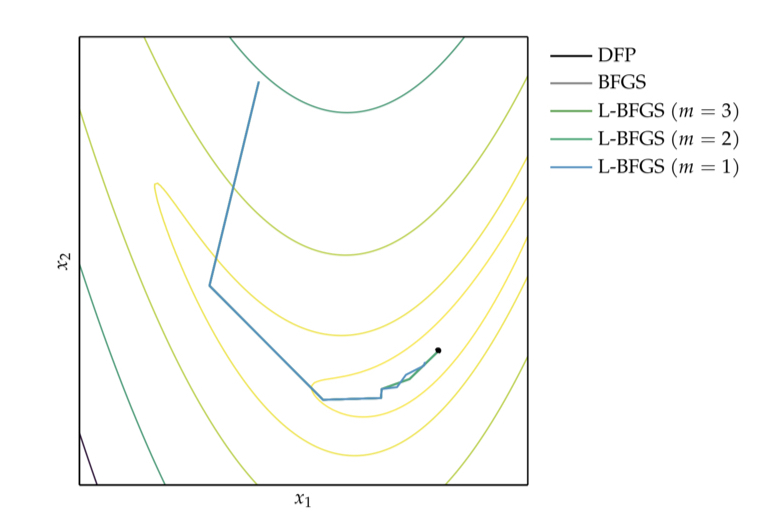
\includegraphics[width=80mm]{Figs/quasi-newton.jpeg}
\end{figure}   
\end{frame}


\section{Summary}
\begin{frame}{Summary}
    \begin{itemize}
        \item Quasi-Newton method attempted to approximate the Hessian from function and gradient evaluations.
        \item The first step approximation of hessian in the quasi-newton methods is usually an identity matrix
        \item BFGS performs better than DFP, but it still relies on the storage of big Hessian matrix
        \item L-BFGS is a more scalable approach for large scale problems.
        \item All quasi-Newton methods can work with the approximate line search.
    \end{itemize}
\end{frame}
\end{document}

